\begin{figure}[htbp]
\centering
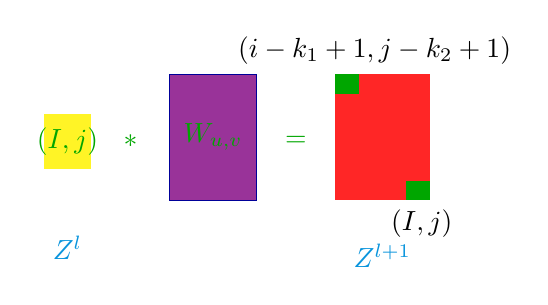
\begin{tikzpicture}[x=1cm,y=1cm]
\fill[yellow!85] (0,.4) rectangle (.6,1.1);\node[green!65!black] at (.3,.75) {$(I,j)$};
\node[green!65!black] at (1.1,.75) {$*$};
\filldraw[fill=violet!80,draw=blue!60!black] (1.6,0) rectangle (2.7,1.6);
\node[green!65!black] at (2.15,.8) {$W_{u,v}$};
\node[green!65!black] at (3.2,.75) {$=$};
\fill[red!85] (3.7,0) rectangle (4.9,1.6);
\fill[green!65!black] (3.7,1.35) rectangle (4,1.6);\fill[green!65!black] (4.6,0) rectangle (4.9,.25);
\node at (4.2,1.9) {$(i-k_1+1,j-k_2+1)$};\node at (4.8,-.3) {$(I,j)$};
\node[cyan!80!blue] at (.3,-.6) {$Z^l$};\node[cyan!80!blue] at (4.3,-.7) {$Z^{l+1}$};
\end{tikzpicture}
\origfig{10}{第 $l$ 个卷积层中像素 $(i,j)$ 与核卷积时，所影响的第 $(1+1)$ 个卷积层输出区域。}
\end{figure}
